\documentclass[border=5pt]{standalone}
\usepackage{pgfplots}
\pgfplotsset{compat=1.18}
\begin{document}
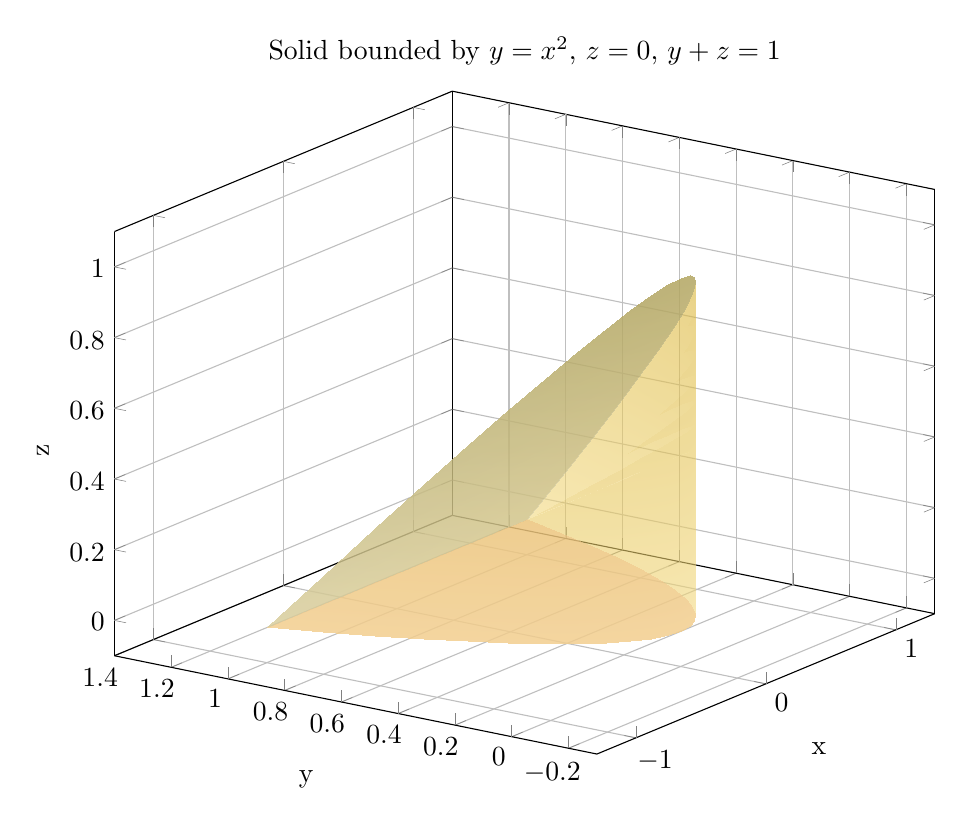
\begin{tikzpicture}
\begin{axis}[
    xlabel={x}, ylabel={y}, zlabel={z},
    xmin=-1.3, xmax=1.3, ymin=-0.3, ymax=1.4, zmin=-0.1, zmax=1.1,
    view={-55}{22},
    width=12cm, height=10cm,
    title={Solid bounded by $y=x^2$, $z=0$, $y+z=1$},
    grid=both
]
% Top surface: z = 1 - y, parametrized over (x, v) with y = x^2 + v(1-x^2)
\addplot3[
    surf, shader=interp, opacity=0.6,
    domain=-1:1, samples=25,
    y domain=0:1, samples y=15,
    colormap={bluewhite}{rgb=(0.6,0.7,0.9); rgb=(0.3,0.5,0.8)}
] ({x}, {x^2 + y*(1 - x^2)}, {1 - (x^2 + y*(1 - x^2))});

% Bottom face z = 0
\addplot3[
    surf, shader=interp, opacity=0.6,
    domain=-1:1, samples=25,
    y domain=0:1, samples y=15,
    colormap={redwhite}{rgb=(0.95,0.7,0.7); rgb=(0.85,0.4,0.4)}
] ({x}, {x^2 + y*(1 - x^2)}, {0});

% Side wall y = x^2
\addplot3[
    surf, shader=interp, opacity=0.6,
    domain=-1:1, samples=25,
    y domain=0:1, samples y=15,
    colormap={yellowwhite}{rgb=(0.95,0.85,0.5); rgb=(0.85,0.7,0.2)}
] ({x}, {x^2}, {y*(1 - x^2)});
\end{axis}
\end{tikzpicture}
\end{document}